%
% graphisch1.tex
%
% (c) 2020 Prof Dr Andreas Müller, Hochschule Rapperswil
%
\begin{figure}
\centering
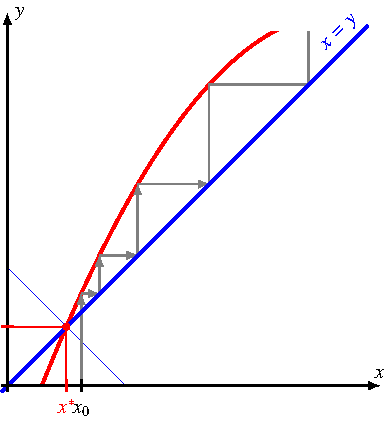
\includegraphics{chapters/10-arithmetik/figures/divergent.pdf}
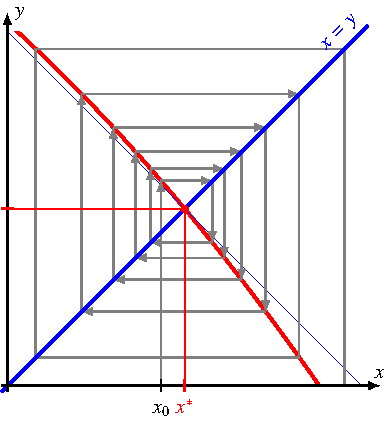
\includegraphics{chapters/10-arithmetik/figures/negdiv.pdf}
\caption{Die Fixpunktiteration $x_{n+1}=f(x_n)$ mit Fixpunkt $x^*$
divergiert für $|f'(x^*)|>1$.
\label{buch:figure:fixpunkt:divergent}}
\end{figure}
